\documentclass[french]{template}

\usepackage{textalpha} % Pour les mots grecs
\usepackage{minted} % Pour le code

\definecolor{LightGray}{gray}{0.9}

\begin{document}
\titre{Projet Immorthon}
\UE{Apprentissage Profond}
\enseignant{Axel \textsc{Carlier}}

\eleves{Alex \textsc{Bechu} \\ Laerian \textsc{Bontinck} \\ Clément \textsc{Demazure} \\ Vianney \textsc{Hervy} \\ Yige \textsc{Yang}}

\fairemarges
\fairepagedegarde
\tabledematieres

\section{Introduction}

Lorsque nous entendons pour la première fois un mot en français, il nous est parfois possible d'en comprendre le sens à l'aide du contexte ou de l'étymologie. C'est cette seconde méthode que nous allons essayer de reproduire à l'aide d'un modèle de language.

\

Les données d'entraînement, le notebook, le script de scrapping et le fichier \texttt{.tex} du rapport sont disponibles sur le dépôt GitHub public du projet\hyperfootnote{https://github.com/sully-vian/immorthon}

\section{Description du sujet}

L'objectif de notre projet tient en peu de mots: \textit{un modèle de langage capable de générer des définitions plausibles pour des mots inventés}.

Toute la difficulté tient dans le terme "définition plausible". En effet, il faut non seulement que le texte généré soit grammaticalement correct et ait la forme d'une définition, mais il faut également que le sens donné au mot soit cohérent avec sa structure étymologique. Par exemple, le mot "étymologie" est formé des radicaux grecs {ἔτυμov} (vrai sens) et {λόγος} (discours). Il est donc logique que sa définition fasse référence à l'étude du "vrai" sens des mots. De manière générale, la plupart des mots scientifiques ont des sens assez clairs pour qui a fait des langues anciennes.

\

Le nom "Immorthon" est un mot-valise entre "immortel" et "python". "Immortel" est le
surnom\hyperfootnote{https://w.wiki/EDk9} donné aux académiciens de l'Académie Française, dont une partie de la responsibilité
est de définir les mots de la langue française.

\section{Données d'entraînement}

Les données nécessaires sont sous forme de paire mot-définition. Le format JSON est parfait pour cela.

Nous avions initialement prévu un corpus de mots en français. En effet, l'orthographe des mots fait souvent explicitement référence à leur étymologie (majoritairement grecque ou latine). Cependant, Il nous fallait aussi trouver un modèle français préentraîné à affiner. Il nous est apparu finalement plus facile de partir d'un modèle anglais et de l'affiner sur un corpus anglais.

\subsection{Corpus}

Différents corpus ont été testés: Les 3000 mots\hyperfootnote{https://www.ef.com/wwen/english-resources/english-vocabulary/top-3000-words/} les plus fréquents en anglais selon le site EF, une liste\hyperfootnote{https://www.mit.edu/~ecprice/wordlist.10000} de 10 000 mots utilisée par un professeur du MIT pour entraîner ses modèles et finalement un corpus de presque 500 000 mots\hyperfootnote{https://github.com/dwyl/english-words}.

\

C'est ce dernier qui a donné les meilleurs résultats. À la fois parce qu'il contient le plus de mots mais aussi parce qu'il contient de nombreux mots rares, scientifiques ou techniques. Un extrait du corpus est donné au listing \ref{listing:corpus}.

\

Sur certains corpus, il nous est apparu que la proportion de prénoms dans notre corpus était anormalement élevée. Environ 10\% des définitions étaient "a first name for boys/girls". Cela a conduit le modèle à souvent reconnaître des mots comme des prénoms. Le corpus finalement choisi n'a que 1\% de prénoms.

\begin{listing}[H]
    \begin{minted}[breaklines,bgcolor=LightGray]{python}
triphthong
serosynovial
syndesmoma
anton
intoxication
vajra
stue
loupcerviers
psychosis
dirtiest
\end{minted}
    \caption{Extrait du corpus (généré avec \texttt{shuf -n 10 words-alpha.txt})}
    \label{listing:corpus}
\end{listing}

\subsection{Définitions}

Une fois le corpus choisi, il nous fallait un moyen de récupérer les définitions des mots. Nous avons choisi de les extraire du site Oxford Learner's Dictionaries\hyperfootnote{https://www.oxfordlearnersdictionaries.com}. Ce choix est dû en partie à la qualité des définitions fournies, à la quantité de mots disponibles et surtout à la facilité de scrapper le site.

\begin{listing}[H]
    \begin{minted}[breaklines,bgcolor=LightGray]{python}
"fornicators","a person who has sex with somebody they are not married to"
"spins","to turn round and round quickly; to make something do this"
"carbonization","the process of becoming or being made into carbon"
"agonies","extreme physical or mental pain"
"militarize","to send armed forces to an area"
"raptor","any bird of prey"
"biding","to stay or live in a place"
"sterility","the fact of not being able to produce children or young animals"
"armada","a large group of armed ships sailing together"
"ambiguities","the state of having more than one possible meaning"
\end{minted}
    \caption{Extrait des définitions (généré avec \texttt{shuf -n 10 dico-alpha.csv})}
    \label{listing:definitions}
\end{listing}

\subsection{Scrapping}

La difficulté principale du scrapping est de comprendre la structure du site. Il faut trouver un algorithme qui fonctionnera pour toutes les pages de définitions. On pense que ces pages sont elles-mêmes générées automatiquement à partir d'un modèle et d'une base de données de définitions. Il est donc possible de rétro-ingéniérer le modèle pour trouver comment extraire une définition d'une page.

Malgré cela, de nombreux mots du corpus choisi ont soit une page dont nous n'avons pas pu extraire la définition, soit n'ont pas de définition sur le site.

Nous nous trouvons donc avec 71010 définitions (7 fois plus que le corpus du MIT), ce qui est suffisant comme nous le verront ensuite.

\

Le résultat du scrapping C++ accéléré par parallélisation OpenMP\hyperfootnote{https://www.openmp.org} est au listing \ref{listing:scrapping}.

\begin{listing}[H]
    \begin{minted}[breaklines,bgcolor=LightGray]{text}
$ ./main corpora/words-alpha.txt dictionnaries/dico-alpha.csv
OpenMP is enabled.
Fetching definitions for 370105 words...
[#########-----------------------------------------] 71010/370105 (19%)
71010 definitions added to dictionnaries/dico-alpha.csv
299095 definitions failed to be added.
Time taken: 18255 seconds.
\end{minted}
    \caption{Résultat du scrapping}
    \label{listing:scrapping}
\end{listing}

\subsection{Préparation des données}

Le modèle doit être entraîné sur des chaines de la forme \texttt{\textless prompt\textgreater\ \textless réponse\textgreater}. Il faut donc unifier les colonnes \texttt{word} et \texttt{definition} de nos données.

\begin{listing}[H]
    \begin{minted}[breaklines,bgcolor=LightGray]{python}
df["text"] = "Define: " + df["word"] + "\n" + df["definition"]
\end{minted}
    \caption{Préparation des données}
\end{listing}

\section{Modèle}

La solution que nous avons choisie pour le modèle de langage est globalement très proche de celle réalisée au TP5 (Transformers pour la génération de texte).

\subsection{Création du modèle}

Nous avons essayé plusieurs modèles préentraînés différents (DistilGPT2\hyperfootnote{https://huggingface.co/distilbert/distilgpt2}, GPT-2\footnote{https://huggingface.co/openai-community/gpt2}).

Le modèle est importé depuis Hugging Face\hyperfootnote{https://huggingface.co/} ou depuis une sauvegarde de notre modèle déjà affiné sur les définitions. Le tokenizer associé est également importé.

On tokenise ensuite la colonne \texttt{text} de notre base de données de définitions. Nous avons choisi un padding de 200 tokens étant donné la répartition des longueurs de définitions (figure \ref{fig:lengths}).

\begin{figure}[H]
    \centering
    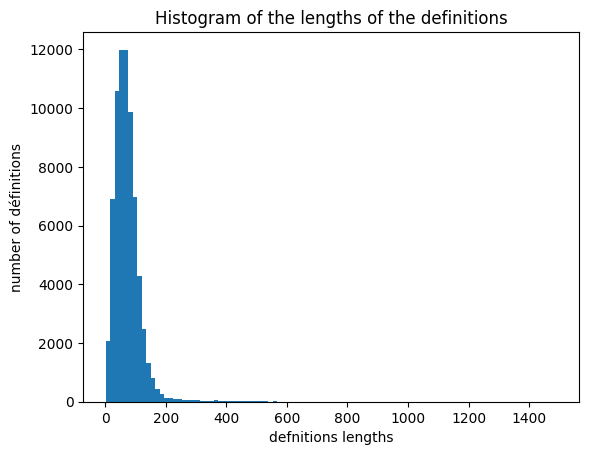
\includegraphics[width=0.7\textwidth]{img/lengths.png}
    \caption{Histogramme de la répartition des longueurs de définitions}
    \label{fig:lengths}
\end{figure}

\subsection{Entraînement}

L'entraînement est réalisé en une seule époque (ou plus si on réentraîne le modèle ultérieurement). La taille du batch est de 8 pour éviter la surchage mémoire des GPU.

Pour le modèle GPT-2, le temps total d'entraînement est d'environ 1h.

\subsection{Utilisation du modèle}

Comme lors du TP5, nous utilisons ici la fonction \texttt{pipeline} de la librairie Transformers pour générer le texte. Le modèle est chargé avec le tokenizer associé.

Le modèle étant entraîné sur des exemples de la forme \texttt{Define: \textless mot\textgreater\textbackslash n\textless definition\textgreater}, il faut donc préparer le prompt d'entrée (listing \ref{listing:generate}).

\begin{listing}[H]
    \begin{minted}[breaklines,bgcolor=LightGray]{python}
def generate(prompt, numDef):
    fullPrompt = f"Define: {prompt}\n"
    results = generator(fullPrompt, num_return_sequences=numDef, ...)
    return [result["generated_text"] for result in results]

for result in generate("zoophobia", 3):
    print(result, end="\n\n")
    \end{minted}
    \caption{Fonction de génération de texte}
    \label{listing:generate}
\end{listing}

\section{Analyse des résultats}

En commençant ce projet nous espérions que le modèle apprenne à reconnaître des préfixes, suffixes et radicaux et à les associer à un sens précis. Cette appproche est parfaitement en accord avec la notion de jetons que le modèle de langage utilise pour générer du texte.

Malheureusement, le fait de patir d'un modèle préentraîné impose le tokeniser et notre affinage ne permet pas de le modifier. Il faut donc se contenter du tokeniseur du modèle de base.

\subsection{Modèle non affiné}

Pour être certain de l'efficacité de notre apprentissage, nous avons réalisé quelques tests sur le modèle GPT-2 non affiné.

\

Le mot \texttt{zoophobia} nous a donné les 2 résultats du listing \ref{listing:zoophobia-raw}. Le premier montre que le modèle croit être au milieu d'un dialogue entre A et B. Il comprend toutefois bien le thème. La seconde génération correspond déjà à ce que l'on aurait pu attendre de notre modèle affiné, mais avec une tendance encyclopédique.

\begin{listing}[H]
    \begin{minted}[breaklines,frame=single,bgcolor=LightGray,linenos]{text}
Define: zoophobia
A: You're a zoo fag, aren't you?
B: No, I'm not.
C: I know.
A: I'm talking about you.
B: Yeah, I'm talking about it.
C: Well

Define: zoophobia
The zoophilia is a condition in which a group of people exhibit behaviors that are considered offensive or offensive. People with a zoophilia typically have difficulty moving around and are often seen in the streets or in parks. The zoophilia can be a sign of a poor judgment,
    \end{minted}
    \caption{Générations du modèle GPT-2 non affiné pour le mot \texttt{zoophobia}}
    \label{listing:zoophobia-raw}
\end{listing}

Pour le mot \texttt{polyphyt} (listing \ref{listing:polyphyt-raw}), la première génération semble correspondre à de la documentation d'une fonction informatique. C'est amusant puisque "polyphyt" est homophone de la fonction "polyfit" de la bibliothèque0 NumPy. La seconde génération laisse penser que le modèle se croit dans la documentation d'un jeu vidéo dont un élément (ennemi, arme, sort...) serait appelé "polyphyt".

\begin{listing}[H]
    \begin{minted}[breaklines,frame=single,bgcolor=LightGray,linenos]{text}
Define: polyphyt
(optional)
The number of times the value of a given value must be specified in any given condition.
The expression
$sum = "1"
will produce the sum of all the values specified in the condition.
Examples
This

Define: polyphyt
Affects: all
Damage Type: damage
Attack Type: movement speed
Attack Speed Modifier: 1.0
Attack Modifier Modifier: 0.9
Shield Modifier: 0.7
Damage Modifier: 0.
    \end{minted}
    \caption{Générations du modèle GPT-2 non affiné pour le mot \texttt{polyphyt}}
    \label{listing:polyphyt-raw}
\end{listing}

\subsection{Modèle affiné}

Le listing \ref{listing:dogoid} nous montre un exemple du modèle qui arrive à décomposer le mot en radical "dog" et suffixe "oid". On peut retrouver dans les données d'entraînement les définitions qui ont pu influencer cette génération: \textit{anthropoid}\footnote{looking like a human}, \textit{spheroid}\footnote{a solid object that is approximately the same shape as a sphere}, \textit{ovoid}\footnote{an object that is like an egg in shape}

\begin{listing}[H]
    \begin{minted}[breaklines,frame=single,bgcolor=LightGray,linenos]{text}
Define: dogoid
having the form of a dog
    \end{minted}
    \caption{Génération du modèle GPT-2 affiné pour le mot \texttt{dogoid}}
    \label{listing:dogoid}
\end{listing}

Le listing \ref{listing:rekiss-antisleep} montre un cas similaire où le sens du mot a été obtenu en isolant des préfixes bien connus ("re-" et "anti-") et en les associant à un radical ("kiss" et "sleep"). Le modèle a donc réussi à comprendre la structure du mot et à en donner une définition cohérente.

\begin{listing}[H]
    \begin{minted}[breaklines,frame=single,bgcolor=LightGray,linenos]{text}
Define: rekiss
to kiss somebody/something again

Define: antisleep
not asleep
    \end{minted}
    \caption{Génération du modèle GPT-2 affiné pour les mots \texttt{rekiss} et \texttt{antisleep}}
    \label{listing:rekiss-antisleep}
\end{listing}

Le listing \ref{listing:siggle} montre un cas particulier où le sens est obtenu par comparaison orthographique avec des mots des données d'entraînement. Les deux premières définitions sont inspirés par \textit{giggle}\footnote{to laugh in a silly way because you are embarrassed or nervous or you think that something is funny} et la troisième par \textit{jiggle}\footnote{to move or make something move up and down or from side to side with short quick movements}

\begin{listing}[H]
    \begin{minted}[breaklines,frame=single,bgcolor=LightGray,linenos]{text}
Define: siggle
to laugh out in a very excited way, especially when you are feeling nervous or have fun

Define: siggle
to let out a soft sound, usually because you are nervous or nervous

Define: siggle
to move or pull somebody/something in different directions
    \end{minted}
    \caption{Génération du modèle GPT-2 affiné pour le mot \texttt{siggle}}
    \label{listing:siggle}
\end{listing}

Le listing \ref{listing:kanyewest} montre un cas où le modèle a réussi à donner le sens d'un terme qui n'a rien à voir avec sa structure étymologique ou avec les mots de son corpus d'entraînement. On remqrque donc que si l'IA a appris le format d'une définition, elle n'a pas perdu les connaissances apprises lors de son entraînement préalable.

\begin{listing}[H]
    \begin{minted}[breaklines,frame=single,bgcolor=LightGray,linenos]{text}
Define: Kanye West
(in the US) a star or a celebrity, especially a famous name

Define: Kanye West
a black and brown American singer, singer, etc.
    \end{minted}
    \caption{Génération du modèle GPT-2 affiné pour le terme \texttt{Kanye West}}
    \label{listing:kanyewest}
\end{listing}

Le listing \ref{listing:empty} montre les résultats obtenus lorsque le prompt à compléter vaut \texttt{Define: \textbackslash n} (aucun mot à définir). On constate que le modèle a appris à générer des définitions même sans mot à définir. Sans rien pour le guider, il génère les définitions les plus génériques possibles. Ce n'était pas forcément prévisible, mais bien cohérent avec son entraînement.

\begin{listing}[H]
    \begin{minted}[breaklines,frame=single,bgcolor=LightGray,linenos]{text}
Define:
a first name for girls

Define:
(in the past) a period of time when the people who lived in the past lived in a different place

Define:
a noun or adjective that has a different meaning
    \end{minted}
    \caption{Génération du modèle GPT-2 affiné pour une entrée vide}
    \label{listing:empty}
\end{listing}

Le listing \ref{listing:encycl} contient des exemples de génération où l'IA a suivit une tendance encyclopédique. Il est en effet souvent difficile de définir un mot sans décrire précisément le concept qui y est associé, raconter son histoire ou expliquer son utilisation. Le problème est que le contexte complet du mot n'est pas nécessairement lié à son étymologie - au contraire de son sens. Le modèlese retrouve donc à inventer des dates, des personnages et des informations complémentaires (tâche bien plus dure que de simplement définir un mot).

\begin{listing}[H]
    \begin{minted}[breaklines,frame=single,bgcolor=LightGray,linenos]{text}
Define: maxitruck
a large vehicle for the driver in the car. A short distance between the driver’s side and the car’s engine makes it more difficult to travel.

Define: UK
East Anglia
(in the UK in the past) the capital of England. It is the largest city, with its large docks and shops. It became an important centre in the 18th and early 19th centuries. It was the capital of the British Invasion in the 18th century and
    \end{minted}
    \caption{Génération du modèle GPT-2 affiné pour les mots \texttt{maxitruck} et \texttt{UK}}
    \label{listing:encycl}
\end{listing}

Le listing \ref{listing:adam} montre un cas particulier de ce qui est présenté au dessus. Avec cette fois la spécificité que le modèle a "puisé" dans les données de son préentraînement pour relier le mot "adam" au personnage de Genèse. On a l'impression d'interroger quelqu'un qui a perdu la mémoire, mais qui accède à des souvenirs très flous et morcelés.

\begin{listing}[H]
    \begin{minted}[breaklines,frame=single,bgcolor=LightGray,linenos]{text}
Define: adam
(16-17) a British man who was sent to fight with God in the Middle Ages. He died in the 4th chapter of the Bible with his wife. His son was the son of Luther.
    \end{minted}
    \caption{Génération du modèle GPT-2 affiné pour le mot \texttt{adam}}
    \label{listing:adam}
\end{listing}

Le listing \ref{listing:blibol} présente un cas rare (rencontré une seule fois sur tous nos tests) où le modèle a inventé\footnote{Le mot "blibo" apparaît sur le wiktionnaire avec une référence vers la page IPA. Cette page concerne l'Alphabet Phonétique International mais peut avoir été interprétée au préentraînement comme la bière IPA, reliant donc avec la définition comme alcool} un second mot ("blibo") afin de définir le premier ("blibol"). Il ne sait donc pas uniquement faire des liens entre un mot prsenté et un mot de sa base de données mais aussi créer un mot qui seraît de la même famille s'il existait.

\begin{listing}[H]
    \begin{minted}[breaklines,frame=single,bgcolor=LightGray,linenos]{text}
Define: blibol
a British company that produces blibos and other alcoholic drinks
    \end{minted}
    \caption{Génération du modèle GPT-2 affiné pour le mot \texttt{blibol}}
    \label{listing:blibol}
\end{listing}

Le listing \ref{listing:non-word} réunit des exemples de génération pour des prompts non-alphabétiques (symboles, chiffres etc). Les résultats ne sont pas décevants du tout. On lit bien que le modèle puise dans les données de son préapprentissage masi respecte bien le format d'une définition.

\begin{listing}[H]
    \begin{minted}[breaklines,frame=single,bgcolor=LightGray,linenos]{text}
Define: 21
21

Define: :)
to say hello, or something in a friendly way

Define: $
a unit of money or a unit of money paid to somebody by a business, school, etc.

Define: %
a unit for measuring the volume or amount of something
    \end{minted}
    \caption{Génération du modèle GPT-2 affiné pour des prompts non-alphabétiques}
    \label{listing:non-word}
\end{listing}

Malgré tous ces résultats intéressants, une part non négligeable des générations sont juste des phrases sans fin qui regroupent des termes liés au sens attendu du mot. Le listing \ref{listing:hallucination} en montre quelques unes.

\begin{listing}[H]
    \begin{minted}[breaklines,frame=single,bgcolor=LightGray,linenos]{text}
Define: eye
the part of the eye that is not there

Define: relooping
to make repeated or repeated a series of repeated or repeated repeated steps

Define: naruto
a first name for boys, short for Jeffrey

Define: blabliblu
a language spoken in a North American people

Define: faker
a person who gives an honest answer to the question that somebody asks

Define: %
the number of people or things that are considered to have a higher than the number of people or things that are considered to have a higher than the number of people or things that are considered to have a higher than the number of people or things that are considered to have a higher than the number of
    \end{minted}
    \caption{Génération du modèle GPT-2 hallucinant}
    \label{listing:hallucination}
\end{listing}

\subsection{Sondage}

En complément de nos analyses, nous avons testé nos définitions à l'aide d'un questionnaire que nous avons fait passer à des amis. Le but était de deviner, pour chaque définition, si elle était issue d'un dictionnaire, générée par une IA, ou inventée par nous. La majorité des participants avaient des connaissances en informatique et en intelligence artificielle.

\

Malgré cela, le score moyen obtenu est de $11,31/20$, ce qui suggère que nos définitions sont globalement crédibles. Une analyse question par question montre que les définitions inventées par des humains sont celles qui ont le plus souvent trompé les répondants. Par ailleurs, certains mots d'argot, comme “dekko : to look at something”, ont une structure syntaxique inhabituelle, ce qui les fait passer pour des inventions, même s'ils sont authentiques.

\

Pour le reste des définitions, les réponses étaient assez équilibrées, autour de la moitié de bonnes réponses. Nous avons également testé ce questionnaire sur ChatGPT (version GPT-4.5), qui a répondu correctement à toutes les questions, identifiant sans erreur les définitions humaines et celles générées par IA.

\

Cependant, le questionnaire présente un biais : en créant nos propres définitions, nous avons tenté d'imiter le style de notre IA. Cela a pu rendre nos définitions plus confuses, ce qui expliquerait les scores plus faibles obtenus pour celles-ci. Il aurait été préférable de séparer le questionnaire en deux parties, ou de se concentrer uniquement sur les définitions générées par IA et celles issues du dictionnaire, afin de mieux évaluer leur crédibilité.

\section{Conclusion}

Ce projet nous a permis de mettre en œuvre un apprentissage supervisé original autour de la génération de définitions pour des mots inventés, en s'appuyant sur leur structure étymologique. L'idée de départ, inspirée des capacités humaines à inférer le sens des mots à partir de leurs racines, s'est avérée pertinente, mais aussi délicate à formaliser pour un modèle de langage.

\

L’une des principales difficultés rencontrées fut la constitution d’un corpus adéquat. Les premiers jeux de données incluaient une forte proportion de prénoms, ce qui biaisait les générations du modèle. Le choix d’un corpus plus large et plus varié, issu d’un dictionnaire anglais, a permis de réduire cet effet, même si des traces de ce biais subsistent dans certaines sorties. Le scrapping des définitions a également représenté un défi technique, que nous avons relevé grâce à un outil en C++ parallélisé avec OpenMP, malgré un taux de réussite limité (environ 19\%).

\

Du point de vue du modèle, l’utilisation de GPT-2 affiné a donné des résultats globalement satisfaisants. Nous avons observé que le modèle réussissait parfois à décomposer les mots en préfixes, radicaux et suffixes pour en tirer du sens — comme avec \textit{dogoid}, \textit{rekiss} ou \textit{antisleep}. Toutefois, les générations restent hétérogènes : certaines sont tout à fait plausibles, d’autres plus encyclopédiques ou incohérentes, et certaines dérivent vers des hallucinations ou des répétitions absurdes. Cela peut s'expliquer à la fois par les limites du tokeniseur, figé par le modèle préentraîné, et par le fait que les mots inventés ne correspondent à rien dans les données d'origine du modèle.

\

Plusieurs pistes d’amélioration s’ouvrent à nous. Sur le plan des données, un filtrage plus rigoureux des entrées (suppression des prénoms, validation de la nature grammaticale) pourrait renforcer la cohérence des définitions générées. En outre, constituer un corpus multilingue ou étymologiquement annoté ouvrirait des perspectives intéressantes, notamment pour entraîner le modèle à associer systématiquement racines et sens. Du côté du modèle, entraîner un tokenizer spécifique ou fine-tuner un modèle multilingue préexistant pourrait améliorer la gestion des néologismes. Enfin, entraîner un modèle de contrôle capable de noter la cohérence d'une phrase pour filtrer les générations hallucinées serait une avancée significative.

\

En somme, si le modèle ne parvient pas toujours à reproduire la finesse humaine dans la compréhension étymologique, il montre des signes encourageants d’apprentissage structurel. L’idée qu’un modèle puisse inventer des mots et leur donner du sens reste une piste prometteuse pour explorer les frontières entre langage, sens et imagination algorithmique.

\section{Annexes}

Quelques générations heureuses que nous n'avont pas pris le temps de commenter

\begin{listing}[H]
    \begin{minted}[breaklines,frame=single,bgcolor=LightGray,linenos]{text}
Define: mythophile
a person who believes that stories and stories are true

Define: mythophile
a person who uses a lot of magic powers

Define: mythophile
a person who believes in the existence of gods and their teachings

Define: hypertoxic
producing a high level of harmful or harmful substances

Define: hopun
a wild tree with a long thick root with leaves often used for making clothes

Define: blibol
to talk in a strange way about your husband, wife or partner, especially when you are feeling ashamed or upset by it
    \end{minted}
    \caption{Générations heureuses du modèle GPT-2 affiné}
\end{listing}

\end{document}